\documentclass[oneside, a4paper, openany]{book}

\usepackage[inner=3cm,outer=3cm,bottom=2cm]{geometry} % Sets the margins of the document
\usepackage[utf8]{inputenc}
\usepackage[british]{babel} % Use British english for hyphenation etc
\usepackage{float} %required for the placement specifier H
\usepackage{tocbibind} % Auto add Bibliography etc to Table of Contents
\usepackage{subcaption} % Creating complex figures
% \usepackage{rotating} % Used to display full page figures
\usepackage[round]{natbib} % Use BibTeX for bibliography management
\setcitestyle{notesep={: }} % Sets the cite separator to column instead of comma
\usepackage{graphicx}
\usepackage{tikz} % Inline drawing
\usetikzlibrary{decorations.pathreplacing}
\usepackage{tabu} % Easier long tables
% \usepackage{url}
\usepackage{makecell} %multi-line cells
\usepackage{hyperref} % Create hyperlinks within text
\usepackage[toc,nonumberlist,nopostdot]{glossaries}
\usepackage{listings} % Source code printer package 
\usepackage{wrapfig}

\makeglossaries % Creates the glossary section
\usepackage{pdfpages} % includes pdf documents
\graphicspath{{./assets/}{./assets/wireframe/}{./assets/design/}}
\begin{document}

\frontmatter
\begin{titlepage}
  \newcommand{\HRule}{\rule{\linewidth}{0.5mm}}
  \center

  \textsc{\LARGE Robert Gordon University}\\[1.5cm]
  \textsc{\Large Bachelor of Science in Computer Graphics and Animation}\\[0.5cm]
  \textsc{\large Honours Project Report}\\[0.5cm]

  \HRule \\[0.4cm]
  { \huge \bfseries A Mobile Application that applies Self-Management Approach to Reduce Sedentary Behaviour}\\[0.4cm]
  \HRule \\[1.5cm]

  \begin{minipage}{0.4\textwidth}
  \begin{flushleft} \large
  \emph{Author:}\\
  Georgi \textsc{Koemdzhiev}
  \end{flushleft}
  \end{minipage}
  ~
  \begin{minipage}{0.4\textwidth}
  \begin{flushright} \large
  \emph{Supervisor:} \\
  Dr. Stewart \textsc{Massie}
  \end{flushright}
  \end{minipage}\\[4cm]

  {\large 2017}\\[3cm]

  \includegraphics[width=5cm, scale=0.1]{rgu-logo.png}\\[1cm]
  \vfill
\end{titlepage}
\chapter{Declaration}
I confirm that the work contained in this Honours project report has been composed solely by myself and has not been accepted in any previous application for a degree. All sources of information have been specifically acknowledged and all verbatim extracts are distinguished by quotation marks.\\[2cm]

  \noindent Georgi Koemdzhiev\\
  5th December 2016
\chapter{Abstract}
Sedentary behaviour is a leading cause of numerous chronic deceases, but currently, there is a lack of mobile applications that try to help tackle this problem. The purpose of this paper is to show how behaviour change techniques can be applied in a mobile application to help people change their sedentary habits. This project proposes a smartphone application that uses daily activity guidelines to increase physical activity. This software will be developed based on findings from background research. It will incorporate behaviour change techniques that will allow maintaining a good goal-performance relationship. Also, self-management logic will be present to facilitate self-care features such as setting a psychical activity goal.
\chapter{Acknowledgements}
Firstly, I would like to express my gratitude to my supervisor Dr Stewart Massie of Robert Gordon University for his guidance during the research and development of the project. \\

\noindent Besides my supervisor, I would like to thank the designers and developers at xDesign for sharing their knowledge and experience with me; my parents Vangel Koemdzhiev and Violeta Koemdzhieva for encouragement me throughout writing this thesis and my partner Mariya Menova for her support and understanding.

% \setcounter{tocdepth}{4}
\tableofcontents
\input{frontmatter/list-of-figures}
\input{frontmatter/list-of-tables}

\newglossaryentry{har}
{
  name=HAR,
  description = {Human Activity Recognition}
}

\newglossaryentry{gsc}
{
    name=GSC,
    description = {Goal-Setting Component}
}

\newglossaryentry{mc}
{
    name=MC,
    description = {Monitoring Component}
}

\newglossaryentry{fc}
{
    name=FC,
    description = {Feedback Component}
}


\glsaddall %Print all entries %
\setglossarystyle{altlist}
\printglossaries

\mainmatter
\chapter{Introduction}
\label{Chapter:Introduction}
Nowadays, with the rapid advance of technology people spend a lot of their time in a static position. According to \citet{wilmot2012} that increases the chances of all-cause mortality by 49\%.  Also, people who lead non-active lifestyle are 112\% more likely to get diabetes, 147\% more likely to experience cardiovascular events, and 90\% more likely to die due to cardiovascular events. 
    
Using self-manageing systems to counter sedentary behaviour is becoming a well-accepted solution due to its many advantages over the traditional paper based methods. This paper proposes a self-management mobile application that apples behaviour change logic to reduce sedentary time as well encourage more physical activity. 
    
    \section{Project Catalyst}
    My passion for software began back in my first year as a student at Robert Gordon University. I was exposed to various modules related to software development which I found absorbing. Consequently, I was able to do a summer internship with a company called xDesign as a Software Engineer and thus gain industry knowledge and skills. I was confident that mobile application development was an area I wanted to pursue. 
    
    This passion for software contributed immensely on the topic of my honours project. Also, the idea of the health aspect of the mobile application made the subject even more appealing to me. My application could potentially help people self-manage their sedentary time as well as promote more physical activity. 
    
    
    \section{Goals and Objectives}
    A set of goals and objectives were formed prior to the initiation of the project to help shape its scope. The goals of the project define the main motivation behind it whereas the objectives underline the main tasks that the project undertakes.
    
    \subsection*{Goals}
    The following project goals have been identified: 
    \begin{enumerate}
        \item Satisfy the requirements the of BSc (Hons) Computing (Graphics and Animation) course
        \item Demonstrate future employers programing as well as UI/UX design skills
        \item Gain a better understanding of how machine learning works 
        \item Go through the main stages of the software development process
    \end{enumerate}
    
    \subsection*{Objectives}
    The following list of objectives helped accomplishing the above goals: 
    \begin{enumerate}
        \item Gather information about Self-Management in the Health sector
        \item Research Sedentary Behaviour factors and consequences
        \item Research behaviour change methods
        \item Research how to implement Human Activity Recognition 
        \item Design and Implement a mobile application on the Android platform based on the project research findings
    \end{enumerate}
    
    \section{Document structure}
    This section of the document addresses how this report is organised.\newline
    
    \textbf{Literature Review} Gives a wide background information regarding using self-management technologies in the health sector, Behaviour changing techniques, consequences and current situation of of Sedentary Behaviour as well as researching commercial and non-commercial HAR mobile applications.\newline
    
    
    \textbf{Specification} Lists the proposed mobile application Functional and Non-functional requirements as well as discussing the system quality attributes. The information in this chapter is heavily influenced by the \textit{Literature Review} chapter.\newline
    
    
    \textbf{Design} Addresses the system design decisions\newline
    
    
    \textbf{Implementation} Details about how the system design have been implemented for each of the main system components.\newline
    
    
    \textbf{Evaluation} A discussing how effective is the implemented system on users.\newline
    
    
    \textbf{Conclusion} Summary of the potential benefits of Sedentary Behaviour self-manageing devices in the health sector, future work and project critical appraisal.\newline
    
    
    \section{Professional, Social, Ethical, Security and legal issues to the project}
    
    \subsection{Professional}
    As a student studying Computing for Graphics and Animations – a course that is accredited by the British Computer Society (BCS) I intend to comply with the BCS Code of Conduct. Specifically point 4 (d) \citep{bcs_2017} - “act with integrity and respect in your professional relationships with all members of BCS…” I intend to acknowledge the authors of any third party software use in this project.

    \subsection{Social}
    The proposed application will try to avoid promoting any body image stereotypes by focusing more on encouraging the users to be more active rather than on their body characteristics such as weight and height or BMI (Body Mass Index). In addition, the application will only show what the recommended activity intervals per day are and will not force the users of the application to follow those strictly (some jobs do require seating for extended intervals of time – e.g. Pilots).
    
    \subsection{Ethical}
    The data collected during the project development such as names of the project participants and their accelerometer sensor data will be stored on disk only for the development purposes of the project. 
    
    \subsection{Security}
    The mobile application, proposed in this work, will offer an authorisation component to prevent other people accessing personal data such as total minutes of activity/inactivity collected daily. What is more, any relevant or valuable user data will be anonymised to protect individual’s identity.

    
    \subsection{Legal}
    To prevent any harm done to the user, the mobile application will show a disclaimer (warning) dialog message to inform the user that they should be in a good physical condition (not suffering from diseases that could lead to worsening the condition of the user) before they use the application. In addition, I intend to fully comply with the terms of conditions of any third party software that I intend to use (my main goal is to use primarily Open Source software). As far as the project participant’s data is concerned, I intend to keep the data only for the purposes of this project, and the data will not be used for any commercial purpose. 

\chapter{Literature Review}
\label{Chapter:Literature-Review}

As it was mentioned in Chapter \ref{Chapter:Introduction} this document proposes a system implemented on a mobile device that encourages the reduction of sedentary time via self-management techniques. In order to gain knowledge on how to devise such as system, literature review needs to be carried away on several topics. First of all, the current shift towards self-management in the health sector will be discussed. The next section will focus on evaluating how much time people spend in Sedentary Behaviour (SB) and what are the consequences. Section 3 looks at digital behaviour change techniques. Commercial and non-commercial \gls{har} mobile applications and \gls{har} itself are discussed in Section 4. Section 5 summarises the system proposed.

\section{Self-Management in the Health Sector}
 \label{section:sm-in-hs}
    Mobile devices with embedded self-management logic are currently being utilised and becoming a well-accepted solution for millions of people in the health sector. For example, the NHS’s England Executive – Simon Stevens, launched a programme “Test Beds” \citep{nhsengland2016,nhsengland2016a} which is a set of collaborative projects between NHS and some technology companies such as Verily, IBM and Philips. The idea behind the project is to test the effectiveness of different technological innovations, including wearable devices and mobile applications. These technologies will enable patients to self-manage illnesses such as diabetes, heart diseases and dementia.
    
    \subsection{Advantages of self-management}
    Shifting towards self-care via mobile devices has many advantages over the traditional methods (e.g., over the phone or face-to-face). For example, self-care devices enable patients to monitor their illnesses at home. \citet[10]{roberts2006} finds that patients using wearables improve their condition and shorten their recovery time if they can be in a familiar environment. Real-time feedback is another advantage of using self-management devices. For example, \citet{alivecor2016}, can prevent critical and even fatal incidents by identifying illness clues ahead of time. Thus, the number of patients becoming seriously ill or needing hospital treatment will potentially be reduced. Consequently, that could save money on hospital treatments \citep{campbell2016}. In addition, \citet[6]{shuger2011} found that real-time feedback on \gls{sb} could be beneficial for weight loss. \citet[97]{whitehead2016} concludes that self-management approaches delivered via mobile applications have the potential to improve outcomes of many chronic diseases.
    
    \subsection{Need for self-management devices}
    It has been found that there is a gap in the current market regarding self-care devices that focus on monitoring \gls{sb} and not only \gls{pa}. For example, \citet{sanders2016} found out that there is a lack of self-management mobile applications or devices on the market that can monitor \gls{pa}. After research, he was able to find 73 devices that provide self-monitoring of PA, and only 9 can monitor sedentary time (see Figure \ref{fig:devices-to-provide-SB-feedback}). That means that there is a lack of products in the market that offer self-management of SB in addition to PA. Sanders also concluded that the current devices capable of measuring sedentary time and providing feedback have not been used in behaviour change interventions. In conclusion, there is a need for further research and development of self-care enabled wearables to help people engage in behaviour change interventions and prevent possible chronic diseases. 
    
    \begin{figure}[h]
        \centering
        \includegraphics[width=10cm]{figureOne}
        \caption{Current technologies that self-monitor and provide feedback on SB \citep{sanders2016}}
        \label{fig:devices-to-provide-SB-feedback}
    \end{figure}

\section{Sedentary Behaviour}

Understanding the consequences of \gls{sb} as well as recommended daily energy expenditure levels is crucial for developing a mobile application that aims to implement behaviour changing theory. It is said that there is a difference between \gls{sb} and \gls{pa} and these terms should be treated differently \citep[540]{networ2012}. For example, a person can do both be sedentary for prolonged periods of time and spend large amounts of vigorous physical activity in one day. Networ define \gls{sb} as “energy expenditure less or equal to 1.5 METs while in a sitting or reclining posture” (see Table 1 for comparison of different activities). As it can be seen from Table \ref{fig:activity-intensities}, the energy spent in static activities does not result in a lot of energy expenditure and that potentially could lead to the occurrence of chronic diseases. \citet[540]{networ2012} also defines a person who is “inactive” as “not meeting specified physical activity guidelines”. That means that a person has to meet the PA recommendation levels in order to be considered as active. The next section will discuss the consequences of SB and the suggested amount of physical activity per day.

    \begin{figure}[h]
        \centering
        \includegraphics[width=10cm]{tableOne}
        \caption{Examples of light, moderate, and vigorous activities \citep{harvardthchanschoolofpublichealth2012}}
        \label{fig:activity-intensities}
    \end{figure}
    
    \subsection{SB consequences and PA recommendations}
    Sedentary Behaviour has been positively associated with diseases such as back pain, diabetes, cardiovascular disease, cancer and all-cause mortality (Wilmot et al., 2012: 2895–2905, Biswas et al., 2015: 123 and Department of Health, 2010: 18). In addition, Biswas et al. (2015: 127) even concluded that SB causes adverse outcomes regardless of the physical activity, although the chances of developing a SB associated chronic diseases are low when involved in higher levels of physical activity.
    
    As far as the PA recommendations are concerned, the Department of Health (2011) and Townsend et al. advocate for 30 minutes of PA for every day of the week. What is more, Parkinson (2016) and Siddique (2016) state that an ideal PA per day would be an hour. Having said that, simply doing 30 minutes or even an hour of activity is not enough. For example, a person may do 30 minutes of activity a day and spend the rest of the time laying or sleeping. To counter that, Swartz, Squires, and Strath (2011) suggest that every static hour should be interrupted by at least of a five-minute walk.
    
    \subsection{Current statistics of sedentary behaviour}
    \citet[19]{townsend2015} found in 2012 that 34\% of adult man and 46\% of adult women did not meet the recommended levels of physical activity. Also, according to \citet[81]{townsend2015}, 45\% of the adults in the UK spend up to 5h and 30 minutes in SB such as watching TV, using a computer or playing video games. What is more, \citet{swinford2014} found in a survey that there has been an increase in the time people spend in sedentary activities compared to 1995. For example, he found that people nowadays take 18 per cent fewer journeys, 24 per cent fewer go to do shopping and 28 per cent visit friends compared to 1995. In conclusion, to improve the state of the people who are spending too much time in sedentary behaviour, there is a need for further research on the effectiveness of behaviour change interventions only focusing on sedentary time and physical activity alone \citep[130]{biswas2015}.

\chapter{Specification}
\label{Chapter:Specification}

The specification of the mobile self-management application can be split into three components: Goal-setting, Monitoring and Feedback. The Goal-Setting Component (GSC), as the name implies, handles setting goals as well as providing additional information such as recommended amounts of physical activity per day. The Monitoring Component (MC) is the most complex part of the system. It is essentially a \gls{har} system with additional logic for recognising the current activity of the user (e.g. walking or static) and logging the data into a database. In addition, this component is responsible for detecting sedentary behaviour and measuring physical activity amounts. As far as the Feedback Component (FC) is concerned, it provides feedback to the user in the form of notifications. 
\section{Functional Requirements}

    \subsection{Goal-Setting Component}
    As it was mentioned in Chapter \ref{Chapter:Literature-Review},  goal-setting is an important part of the behaviour change process. It allows the user to set goals which is the first step towards better lifestyle. This component's requirements are mainly derived from the background research. 
    
    \begin{enumerate}
        \item \gls{gsc} shall allow the user to set \gls{pa} goals
        \begin{enumerate}
            \item \gls{gsc} shall provide list of recommended \gls{pa} goals
            \item \gls{gsc} shall allow the user to set custom \gls{pa} goals
        \end{enumerate}
        \item \gls{gsc} shall allow the user to set Sedentary Time (\gls{st}) goals
        \begin{enumerate}
            \item \gls{gsc} shall allow the user to set the maximum duration of \gls{st} before a reminding notification is sent 
        \end{enumerate}
    \end{enumerate}
    
    
    \subsection{Monitoring component}
    The main purpose of the \gls{mc} is to continuously recognise activities and analyse the levels of \gls{pa} and \gls{st}. The following requirements have been derived from analysing past and current mobile devices and applications.
    
    \begin{enumerate}
        \item The \gls{mc} component shall classify physical activities
        \begin{enumerate}
            \item HAR component shall recognise the following activities:
            \begin{enumerate}
                \item walking
                \item running
                \item cycling
                \item static
            \end{enumerate}
        \end{enumerate}
        \item The \gls{mc} component shall analyse user's \gls{pa} and \gls{st} amounts in real time
            \begin{enumerate}
                \item \gls{mc} shall increment user's \gls{pa} or \gls{st} value whenever physical activity or sedentary behaviour is recognised
            \end{enumerate}
        \item The \gls{mc} shall personalise \gls{har}'s classifier
            \begin{enumerate}
                \item When enough user data is collected, the system shall retrain the classifier with user's own data
            \end{enumerate}
            
        \item \gls{mc} shall keep history of previously accumulated \gls{pa} and \gls{st} amounts
        
        \item The user shall be able to set "Sleeping Hours", time interval during which no measurement of \gls{pa} or \gls{st} should occur
      
    \end{enumerate}
    
    \subsection{Feedback Component}
    The \gls{fc} is responsible for sending notifications to the user. It can provide important information such as when a previously set goal is attained or reminder for the user that they are spending too much static time.
    \begin{enumerate}
        \item \gls{fc} shall notify the user when they are being sedentary for too long (e.g. an hour)
        
        \item \gls{fc} shall notify the user when a previously set goal is attained (e.g. being active for 30 minutes)
        
        \item \gls{fc} shall not send notifications during "Sleeping Hours" time interval
    \end{enumerate}

\section{Non-functional Requirements}
The mobile application proposed in this work has to comply to a number of additional requirements. Since the \gls{gsc},\gls{mc} and \gls{fc} are all part of the same software, their non-functional requirements will be discussed all together.
    
    % \subsection{Limitations}
    
    \subsection{Accuracy}
    The accuracy of the system shall be high so that misclassification of activities are avoided or minimised. For example, classifying "walking" as "static" would lead to incorrect \gls{pa} daily readings. Consequently, the user may be doing less physical activity if they are notified they attained a goal.
    
    \subsection{Battery consumption}
    Since the resources of every portable device (i.e. mobile phone) are constrained, the system shall be designed so that it consumes reasonable amount of battery power. For example, the user must not need to charge the device in the middle of the day since that renders measuring component of the application useless (the application cannot measure \gls{pa} when the device is on the user).
    
    \subsection{Security}
    The mobile application shall store user data only on the system in order to minimise the risk of data breach. In addition, the following considerations have been taken into account:
    
    \begin{enumerate}
        \item The system shall provide protection of user's data
            \begin{enumerate}
                \item The system shall show authentication screen before showing any sensitive data
                \item The system shall encrypt the data stored in a local database
            \end{enumerate}
    \end{enumerate}
    
    \subsection{System Quality Attributes}
        
        \subsubsection{Adaptability}
        Modern mobile applications should be able to quickly adapt to new requirements as the market always changes. That is why the system design implements the \gls{mvp} software pattern which increases the ability of the system to incorporate new features easily.
        
        \subsubsection{Scalability}
        It is difficult to envision how much data will be gathered from the sensors of the smartphone. However, the system should be scalable and thus capable of handling large amounts of computations.
        
        \subsubsection{Modularity}
        The system is comprised of different units. For example, each screen is encapsulated in a separate directory which can be interchanged easily without changing the integrity of the system.  
        
        \subsubsection{Testability}
        To assure that the system works as intended, the system shall be tested by both assertions and Quality Assurance tests. 
        
        \subsubsection{Maintainability}
        The system shall be designed in such a way so that it allows for easy debugging and evolution. For example, extending the system by adding new features.
        
        \subsubsection{Robustness}
        The system will constantly work in the background (e.g. collect contextual data) so ensuring that the system encompass as many points of failure as possible is crucial.
    
    
    
\chapter{Design}
\label{Chapter:Design}

This chapter discusses the design considerations taken during the design development of the system. The design stage is very important since it lays down the foundation for the whole system. If not done right it could lead to undesired consequences later on in the implementation stage and even in the end-product. \citet[12]{bell2005} states that about 5\% of the total time that takes for the development of a software should be spent for the design state alone. For comparison, the coding takes about 7\% and Testing takes 8\%. Thus a considerable amount of time has been spent in designing the system. 

The design process has gone through many iterations to ensure the best possible quality of the product. The design can be split into two main sections, namely User Interface (UI) Design and System Architecture (SA) design.
\chapter{Development Methodologies}
\label{chapter:development_methodologies}
This chapter discuses the development practices that are used during the development process of the proposed system.  

\section{Development Model}
\label{section:development-model}
As with every software product, specific rules are needed to ensure that the software is developed in a manner that satisfy its specifications and achieves the end-goals. In the IT industry that is achieved by following a software development model. It specifies the required stages of the development and the order in which the they are carried out. In this project the \textit{Incremental Model} has been chosen to drive the development of the software. The main idea behind this model is developing a system through iterative steps and in small incremental portions \citep[264]{bhuvaneswari2013}. It ensures that each iteration (e.g. software build) is tested and working before using the previous iteration as a bases for the next one (see figure \ref{fig:incremental-model}). The The main benefits of using this model are:

\begin{itemize}
    \item A product is produced early in the project's development
    \item Because of the previous point, unforeseen problems can be detected early
    \item Client change requests can be implemented between increments
\end{itemize}

    \begin{figure}[H]
        \centering
        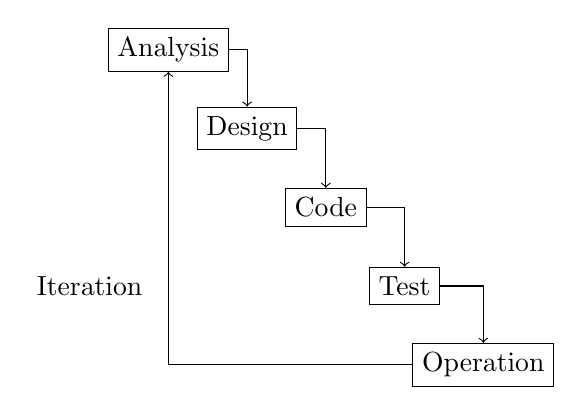
\begin{tikzpicture}
            % nodes
            \node (a1) [draw]  {Analysis};
            \node (d1) [draw, below of=a1, right of=a1] {Design};
            \node (c1) [draw, below of=d1, right of=d1] {Code};
            \node (t1) [draw, below of=c1, right of=c1] {Test};
            \node (o1) [draw, below of=t1, right of=t1] {Operation};
            \node at (-1,-3) {Iteration};
            % arrows
            \draw[->, to path={-| (\tikztotarget)}](a1) edge (d1) (d1) edge (c1) (c1) edge (t1) (t1) edge (o1) (o1) edge (a1);
        \end{tikzpicture}
        \caption{Incremental software development model life cycle}
        \label{fig:incremental-model}
    \end{figure}


\section{Version Control System}
When developing a software challenges can occur unexpectedly and a developer has to do whatever possible to ensure the their work is protected. For example, untraceable bug can be introduced in one of the iterations of the iterative development model (see section \ref{section:development-model}) that could lead to poor system performance. In order to prevent the (or at least dramatically lower)the occurrence these situations the use of \textit{"Version Control"} is encouraged.

There are many Version Control Systems (VCS) out there such as Mercurial, Fossil and Git. The main purpose of a \gls{vcs} is to keep track of the changes in a project. If a developer is satisfied with a specific change, they can perform a \textit{commit}. That action will merge the change to the codebase and the commit command will be added to the changelog (list of commits). If there is a problem that has been caused by a previous \textit{"bad"} commit, the developer can simply revert the whole project to a more stable state by restoring the codebase to a previous known \textit{"good"} commit.

For this project, Git has been chosen along with its web service GitHub\footnote{\url{https://github.com}} to serve as a \gls{vcs} due to the fact that it is easy to use and it is well-documented.


\section{Project Management}
It is important to stay organised when it comes to working on a project, especially when it involves the usage of limited resources (i.e. Time). Thus, a project management tool called \textit{Taiga.io}\footnote{\url{https://taiga.io}} was utilised to help keep track of the project's progress via \textbf{\textit{Kanban} boards}. With every incremental iteration (see \ref{fig:incremental-model} above) new tasks are identified, created and added to the Kanban boards.

Using \textit{Kanban} boards introduces several benefits to the development of the project. Firstly, it provides a quick way to organise the project work visually. For example, boards titled \textit{"READY"} and \textit{"IN PROGRESS"} tables contain that tasks that are already implemented and what those that are being implemented, respectively (see figure \ref{fig:taiga-kanban-boards}). Secondly, it increases the development efficiency since one of the key aspects of the Kanban methodology is to limit the work in progress (WIP) by setting a limit \citep[]{atlassian2017}. For example, if the number of tasks in \textit{IN-PROGRESS} board is 1, that means that no other tasks should be started until the currently undergoing one is finished.

\begin{figure}[ht]
    \centering
    \includegraphics[width=15cm]{taiga-kanban-boards}
    \caption{Taiga Kanban boards}
    \label{fig:taiga-kanban-boards}
\end{figure}

\section{MVP and Dependency Injection}
    As discussed before, the implementation of the mobile application is following the \gls{mvp} software pattern, which allows for the clear separation of code concepts (see section \ref{section:architectural-design}). To better satisfy the requirements discussed in section \ref{section:system-quality-attributes}, \gls{mvp} is combined with a Dependency Injection (DI) principle. What \gls{di} do is shifting the responsibility of one class to create its dependencies to another class. For example, class Car requires class Engine as a parameter. Instead of creating a new instance of class Engine when class Car is created it is simply provided as a constructor parameter in class Car's constructor (see listing \ref{di-car-example}).
    
     \begin{wrapfigure}{RI}{0.3\textwidth}
        \begin{center}
            \includegraphics[width=0.3\textwidth]{app-directory-structure}
        \end{center}
    \caption{Data collection screen directory structure}
    \label{fig:app-directory-structure}
    \end{wrapfigure}
    
    Dagger\footnote{\url{https://github.com/google/dagger}} is a framework that utilises the \gls{di} principle in the form of \textit{Component} and \textit{Module} classes. A module creates the necessary dependencies (e.g. object of class B) whereas the Component class determines where those dependencies will be "injected" (e.g. satisfy dependence's in class A). A concrete example of \gls{di} can be seen in Listing \ref{di-example}. In this example, the \textbf{LoginFragment} (e.g. the login screen) requires an object of type \textit{\textbf{"ILoginPresenter"}} to function. The method \textit{\textbf{"satisfyDependencies()"}} provides the dependencies to the class (e.g. externally). All of the dependencies of the Login screen are provided from a Dagger module named \textit{\textbf{"AuthModule"}} which is responsible for providing and creating the concrete implementation of the above interface (e.g. ILoginPresenter). The full code of \textit{\textbf{"AuthModule"}} as well as \textit{\textbf{"AuthComponent"}} can be seen in Appendix \ref{chapter:dagger-component-module}.  
    
        
    Combining the \gls{mvp} design pattern with dependency injection framework such as Dagger brings a lot of advantages for the software product. Firstly, the software becomes more loosely coupled as the \gls{mvp} enforces the use of interfaces and Dagger is responsible for injecting the concrete implementation of those interfaces where required. Secondly, it allows for logically structuring the codebase. For example, a common approach when using both \gls{mvp} and Dagger is to create a directory for each one of the mobile screens (see figure \ref{fig:app-directory-structure}) containing the necessary \gls{mvp} classes such as \textit{\textbf{Presenter}} and \textit{\textbf{Model}} and the as well as Dagger's \textit{\textbf{Module}} and \textit{\textbf{Component}} to handle the \gls{di} process.
    
\begin{lstlisting}[caption= DI example, label=di-car-example,frame=tlrbr,basicstyle=\small,captionpos=b]
    class Car{
        Engine engine;
            Car(Engine engine){
                this.engine = engine;
            }
       }
    }
\end{lstlisting}

\chapter{Implementation}
This chapter discusses the implementation details of the proposed mobile application. First, the \gls{har} stages will be discussed. That includes the data gathering from the projects' participants as well as data prepossessing and training a classifier. Next, the specifics of the mobile application itself will be discussed such as database and overall system design implementation.

\section{The mobile application}
          
    
    \subsection{Realm Database}
    
    \subsection{Data collection service}
    
    \subsection{Active Minutes service}
    


\section{Human Activity Recognition}
In order for the system to take actions such as notifying the user for a prolonged periods of inactivity or sending a notification when a \gls{pa} goal is achieved, the application needs to recognise human activities (i.e. walking and running). Implementation of the \gls{har} system will be discussed bellow.

    \subsection{Data Collection}
    One of the key stages in the development process of a typical supervised (online) \gls{har} system is the data collection stage. A labelled dataset is needed in order to train a model (or also called classifier). The produced model can classify an "unseen" (or unlabelled) data to a specific activity (i.e. walking or being static).
    
    \subsubsection*{Setting and project participants}
    The data needed to train the model in this work was collected from 3 fellow students in a controlled environment. Each one of the project participants was equipped with a device running partially implemented \textit{"Active Minutes"} application (e.g. only the \textit{"Data Collection screen"} see \ref{fig:data-collection-screen-design}). Before performing the data collection process, the participants had to, first, select the activity they will perform from a list of activities and then press the Start button on the application's UI in order to start the data collection process. The location of the device during the recording was chosen to be the front pants pocket. This location has been found to be the optimal position for \gls{har} (see \ref{section:non-commercial-har-systems}). All of the participants recorded 3 minutes of each one of the following activities: \textit{walking}, \textit{running}, \textit{cycling} and \textit{static}. To avoid any unwanted information during the recording stage, the first and the last 7 seconds of each activity was removed since it contained noise information such as the linear acceleration taking place when the device was put in and pulled out of participants pockets. That was pragmatically done and no direct human intervention was needed to further filter the data.
    
    \subsubsection*{Recorded data}
    \label{subsubsection:recorded_data}
    When all of the required data was collected, it was converted into a WEKA ARFF file format by pressing the "EXPORT" button on the Data Collection screen. The ARFF file was stored on the device's external memory (e.g. SD card). A sample of the produced ARFF file can be seen in Listing \ref{weka-arff-code}. A dataset containing ~720 labelled data points (or a total of ~36 minutes of data) was produced as a result of the data collection process. 
    
   
    
\begin{lstlisting}[caption=WEKA ARFF file extract,
label=weka-arff-code,captionpos=b, frame=single,basicstyle=\small,float,floatplacement=H,breaklines=true]
@relation HAR
    
@attribute accX__fft1 numeric
@attribute accX__fft2 numeric
@attribute accX__fft3 numeric
@attribute accX__fft4 numeric
@attribute accX__fft5 numeric
@attribute accY__fft1 numeric
@attribute accY__fft2 numeric
@attribute accY__fft3 numeric
@attribute accY__fft4 numeric
@attribute accY__fft5 numeric
@attribute accZ__fft1 numeric
@attribute accZ__fft2 numeric
@attribute accZ__fft3 numeric
@attribute accZ__fft4 numeric
@attribute accZ__fft5 numeric
@attribute accM__fft1 numeric
@attribute accM__fft2 numeric
@attribute accM__fft3 numeric
@attribute accM__fft4 numeric
@attribute accM__fft5 numeric
@attribute class {walking,running,static,cycling}
    
@data
9,-76,-834,25,22,4,-1,-401,-190,-3,3,5,-213,-94,-45,2,-50,-49,-15,18,walking
-0,-184,140,4,-34,-2,13,45,63,-8,0,51,-68,-30,-72,1,-52,15,-51,63,walking
-1,-13,-30,3,2,3,-18,-2,3,-21,-1,2,-4,-9,-1,-2,33,3,16,20,walking
0,-16,-17,-22,6,-3,-6,-8,-16,-3,-15,-2,12,-5,9,8,8,37,38,-18,walking
-6,-22,14,-54,1,14,8,27,9,60,-22,-31,-11,-11,4,-7,1,0,-3,-39,running
-3,-11,-35,-3,-53,-13,-45,23,-57,17,-2,52,13,58,15,22,48,-36,25,-50,running
3,7,-11,27,-41,-19,-31,-53,-107,10,0,-42,22,-42,3,20,34,-26,76,-104,running
-3,37,34,9,58,0,30,97,-74,83,4,-13,-39,40,26,-4,15,-10,27,-26,cycling
-1,-91,-131,-121,-58,-4,6,-66,22,70,3,-30,-76,-63,-30,-1,-39,-10,-39,-76,cycling
1,-54,-41,-180,114,-3,4,-21,78,-188,3,8,-56,-19,70,0,-38,22,-83,103,cycling
0.3,0,-1,1,-1.4,0,1,-1,0,0,0,-1,0,0,0,0,0,0,0,0,static
0,-6,48,-8,0,0,-6,-21,2,5,0,-1,42,-6,0,0,0,-1.5,0,-1.6,static
-0.3,8,-4,3,-4,0.1,6,-4,2,-3,0,2,-2,2,-1,0,0.2,1,-0.4,0.2,static
\end{lstlisting}
    
    The device used to collect the data was \textit{OnePlus One} equipped with low-power high performance 3-axes accelerometer \footnote{\url{http://www.st.com/en/mems-and-sensors/lis3dh.html}}. As for the sampling frequency (SF) of the sensor, the Android Operating system provides a total of four different sampling frequencies for reading the accelerometer sensor, namely \textit{NORMAL: 5 Hz}, \textit{UI: 16 Hz}, \textit{GAME: 50 Hz}, and \textit{FASTEST}. The latter has been chosen for the SF of the built-in accelerometer as it has produced good results in \citet[3-5]{lee2016}. According to the Google's documentation \textit{FASTEST} SF depends on the hardware of the device \citep{googlesensormanager2017}. In this case, the SF was \textbf{115} Hz. 
    
    \subsection{Training the kNN classifier}
    The exported ARFF Weka file (see section \ref{subsubsection:recorded_data}) is then bundled into the application itself by transferring the collected data straight into the \textit{Assets} directory of the mobile application. That allows for "shipping" the application with the collected training dataset. The \gls{knn} classifier is then trained and serialised when the \textit{onCreate} method of the \textit{Application} is called. This method is only called once during the life of the application \citep{googleapplication2017}.
    
    \subsubsection*{Accuracy}
    The ARFF Weka file (dataset) was tested externally on a PC to find the optimal \gls{knn} parameters such as the number of neighbours the classifier should consider before making a class prediction as well as whether to perform a cross validation of the data. The testing was done using the PC version of WEKA \footnote{\url{http://www.cs.waikato.ac.nz/ml/weka/}} Machine Learning application. After performing thorough testing, the default parameters of the \gls{knn} classifier performed the the best reaching accuracy of \textit{83.7\%} for dataset containing 763 data points. The performance for the trained model can be seen in table \ref{table:4_class_confusion_matrix}. 

\begin{table}[ht]
\centering
\begin{tabular}{ |c|c|c|c||c| } 
 \hline
 a & b & c & d & classified as\\
 \hline \hline
 140 & 4 & 2 & 33 & a = walking \\
 57 & 112& 0 & 10 & b = running \\
 0 & 1 & 218 & 0 & c = static \\
 5 & 1 & 11 & 169 & d = cycling \\
 \hline
\end{tabular}
\caption{4 classes Confusion Matrix}
\label{table:4_class_confusion_matrix}
\end{table}

According to the confusion matrix in the table above, data points of class "running" has been incorrectly classified 57 times as class "walking" and 10 times as class "cycling". However, for the implementation purposes of the proposed application that performance of the model is still acceptable because even though the classifier has been designed to distinguish between 4 classes, only 2 classes are taken into account, namely "static" and "active" (including "walking", "running" and "cycling") on a programming level. Feature versions of the application may utilise the "active" classes to show a more detailed information to the user such as how much time the user has spend walking or running throughout the day.

To demonstrate the actual accuracy of the model taking account only those 2 classes, the original dataset has been modified so that only 2 classes are present - static and active. The confusion matrix after training the model(again the same \gls{knn} classifier with default parameters) can be seen in table \ref{table:2_class_confusion_matrix}. The actual accuracy of the classifier reaches 98.1\% since only 14 data points has been incorrectly classified.

\begin{table}[ht]
\centering
\begin{tabular}{ |c|c|c| } 
 \hline
 a & b & classified as\\
 \hline \hline
  531 & 13 & a = active\\
  1 & 218 & b = static\\
 \hline
\end{tabular}
\caption{2 classes Confusion Matrix}
\label{table:2_class_confusion_matrix}
\end{table}
    
    \subsection{HAR System Implementation}
    The basic structure of the \gls{har} system integrated into the application has been informed by \citet[149]{labrador2013}. For example, the measurements of the accelerometer sensor in a given time can be represented pragmatically by a class \textit{Point} containing class fields such as "time" and "value". A simplified diagram of the \gls{har} system can be seen in figute \ref{fig:har_system_impl_class_diagram}.
    
    \begin{figure}[ht]
        \centering
        \includegraphics[width=13cm]{har_system_class_diagram_pdf}
        \caption{HAR system class diagram (simplified)}
        \label{fig:har_system_impl_class_diagram}
    \end{figure}
    

\section{Self-Management System Implementation}



    
    
    
    
\chapter{Testing and Evaluation}
\label{chapter:testing-and-eval}
The purpose of this chapter is to evaluate how effective is the developed mobile application in respect to applying the behaviour change theory discussed in Chapter \ref{Chapter:Literature-Review}. To examine that, a series of tests were performed, namely \textit{Acceptance}, \textit{Functional} and \textit{Usability} testing. Furthermore, a survey was carried out on three university students in order to obtain general user opinion regarding varying aspects of the application. The tests performed on the system are going to be discussed first followed by a discussion on how the system compares with a current commercial product in the same field. Finality, the survey responses are examined.

\section{Acceptance Testing}
Acceptance testing is a key part of the software development process. It evaluates weather the software conforms with the client requirements. Consequently, it is determined if the end-product is capable of performing the specified functionality. The following sub-components of the system underwent Acceptance testing, namely \textit{Goal-Setting Component} (\gls{gsc}), \textit{Monitoring Component} (\gls{mc}) and \textit{Feedback Component} (\gls{fc}).

\subsection{Goal-Setting Component}
All of the three specifications for this component were implemented successfully. The list of the implemented requirements can be seen in Appendix \ref{chapter:am-acceptance}.

The first requirement - "\gls{gsc}" shall provide list of recommended \gls{pa} goals - was implemented by utilising an Android framework component called \textit{Dialog} \citep{androiddialogs_2017}. A Dialog window is presented to the user so they can choose their \gls{pa} goal in minutes (e.g. 10, 20, 30, 60).

The second requirement \textit{"\gls{gsc} shall automatically set the recommended \gls{pa} goal if the user does not explicitly do so"} is implemented in the \textit{initial setup} set of screens discussed in section \ref{section:initial-setup-screens}. If the user decides to skip the \textit{initial-setup} screens (which offer options such as setting the \gls{pa}, \gls{mci} and the \textit{Sleeping Hours} time interval) default values are set. For example, the \gls{pa} goal is set to 30 minutes, \gls{mci} (or the \gls{st} goal) is set to 60 minutes and the \textit{Sleeping Hours} time interval is set to 8pm to 8am.

The third and last requirement "\gls{gsc} shall allow the user to set a Maximum Continuous Inactivity (MCI)..." was successfully implemented using a dialog window. It allows the user to set their \gls{st} (or \gls{mci}) goal by selecting it from a list of preset values in the dialog. In addition to the \textit{initial setup} screens the user is able to do that in the \textit{Settings} screen. 

\subsection{Monitoring component}
Four out of the five initially set features were fully implemented. The list of the implemented requirements can be seen in Appendix \ref{chapter:am-acceptance}.

First of those features \textit{HAR component shall recognise 4 activities(walking, running, cycling and static)} was implemented by gathering activity data from fellow university students and training a classifier to recognise the above-mentioned activities.

As far as \textit{\gls{mc} shall increment user's \gls{pa} or \gls{st} value whenever physical activity or sedentary behaviour is recognised} is concerned, this feature was implemented in the \textit{ActivityMonitor} class (see section \ref{section:activity-monitor}). This class is responsible for incrementing the activity and inactivity values depending on the recognised class by the classifier.

\textit{The system shall allow the user to group the collected data in "Daily" and "Weekly" representation}. This feature was implemented in the \textit{History} screen of \textit{ActiveMinutes}. The \gls{ui} of this screen includes \textit{DAILY} and \textit{WEEKLY} buttons allowing the user to switch between both representation of the collected data, accordingly.

The next requirement - \textit{The user shall be able to set the \textit{Sleeping Hours} time interval during which no measurement of \gls{pa} or \gls{st} should occur} - was implemented in the \textit{Settings} screen. The \gls{ui} of this screen provides the user with the option to change their \textit{Sleeping Hours} time interval by tapping on the appropriate menu item and choosing the desirable start and end times.

There were some features of the system that were not implemented since it was determined to be too complex given the project time constrains. One of those feature was \textit{The \gls{mc} shall personalise \gls{har}'s classifier}. This feature was discussed in section \ref{section:classifier-personal-service} and it has been designed as Android \textit{Service}. It uses the gathered-with-time and filtered by the classifier's confidence level data (e.g. above 80\% - to filter only the recognised activities with high confidence). The service combines this data with the general one and produces a personalised model that is used for further classification. According to \citet[376]{arapakis_athanasakos_jose_2010}, that is expected to improve the classifier's accuracy.

\subsection{Feedback Component}
As far as the \gls{fc} is concerned, a total of three features were successfully implemented. One of the initial requirements of the \gls{fc} was not implement due to the project's time constrains. \textit{FeedbackProvider} (see section \ref{section:feedback-provider}) represents the \gls{fc} implementation system-wise.

The first requirement - \textit{\gls{fc} shall notify the user when they are being sedentary for 1 hour} allows the user to be notified for a prolonged sedentary time. This feature was implemented by utilising Android's \textit{Notification} API. In addition, this API is used to satisfy another feature as well, namely \textit{\gls{fc} shall notify the user when a previously set goal is attained}. It allows the user to be notified when they achieve their daily goal (e.g. 30 minutes of \gls{pa}).

Another feature implemented feature - \textit{\gls{fc} shall not send notifications during the user set "Sleeping Hours" time interval} makes sure that the system stops monitoring user's \gls{pa} and \gls{st} levels when \textit{Sleeping Hours} time interval is entered. 

Last but not least, \textit{\gls{fc} shall send a notification to the user every Sunday to show goal-performance feedback for the past week} - a feature (or rather screen) which provides more information to the user regarding their goal-performance in comparison the only receiving notifications. Although "good-to-have", this feature was not implemented due to the project's time constrains rather than lack of technical capability. The list with all of the requirements of this component can be seen in Appendix \ref{chapter:am-acceptance}.

\section{Functional Testing}
This is a quality assurance (QA) test aiming to verify that the system is providing the same output as required by the end user. Each test has an input, expected result, actual result and states whether the system passes the test or not.

Every feature of the system was tested to ensure that it works and satisfies the functional requirements of the system. For example, test cases verified that if the navigation of the system works as expected e.g., when the user preses the \textit{History} menu item of the navigational drawer, that takes the user to this screen. In addition, self-management was tested as well e.g., the goal-setting, monitoring and feedback components. For example, to test the monitoring component of the system the user (one of the project participants) had to perform 5 minutes of \gls{pa} or \gls{sb}. The result was compered with the \textit{Actual result} (if the system measures successfully the above amount). A snippet of the monitoring component functional testing can be seen in Table \ref{tab:monitoring-com-ft}.

\begin{table}[ht]
    \centering
    \fontsize{9}{12}\selectfont
    \tabulinesep=1mm
  \begin{longtabu} to \textwidth {|l|X|X|X|l|l|}
    \hline
      \textbf{Step No}
      & \textbf{Test Cases}
      & \textbf{Expected result}
      & \textbf{Actual result}
      & \textbf{Status}
    \endhead \hline
    1
    & \raggedright The user starts the mobile application and performs 5 minutes of \textbf{walking}.
    & \raggedright The system should recognise that the user is performing \gls{pa} and increments \textit{Active} time. 
    & \raggedright Works as expected e.g., updates the \gls{ui} by adding 5 minutes to the \gls{pa} progress bar in \textit{Today} \& \textit{History} screens.
    & Pass
    \\ \hline
    2
    & \raggedright The user starts the mobile application and performs 5 minutes of \textbf{running}.
    & \raggedright The system should recognise that the user is performing \gls{pa} and increments \textit{Active} time. 
    & \raggedright Works as expected e.g., updates the \gls{ui} by adding 5 minutes to the \gls{pa} progress bar in \textit{Today} \& \textit{History} screens.
    & Pass
    \\ \hline
\end{longtabu}
    \caption{Monitoring activity functional test snippet}
    \label{tab:monitoring-com-ft}
\end{table}

A total of 30 test cases in different categories were created to ensure that every implemented feature of the system is tested. The system successfully pass all of the tests. The device used during the tests was \textit{Google Pixel} \footnote{\url{https://madeby.google.com/intl/en_uk/phone/}}. All test cases can be seen in Appendix \ref{chapter:functional-testing}.

\section{Usability Testing}
In addition to the above-mentioned types of testing, usability testing has been performed on the system to determine if it is easy to use. To determine that the usability test consisting of 16 tasks that the a real user (i.e., one of the project participants) performed on the system. A snippet of the usability test can be seen in Table \ref{tab:usability-test-snippet}. The full list of the tasks can be seen in Appendix \ref{chapter:usability-testing}.

\begin{table}[ht]
    \centering
    \fontsize{9}{12}\selectfont
    \tabulinesep=1mm
  \begin{longtabu} to \textwidth {|l|X|X|l|}
    \hline
      \textbf{Task No}
      & \textbf{Task}
      & \textbf{Comments}
      & \textbf{Status}
    \endhead \hline
    1
    & \raggedright Open the application and create an account.
    & \raggedright The user was able to understand what was required and complete the process by accessing the Sign-up screen, entering their credentials and selecting the \textit{SIGN UP} button.
    & Pass
    \\ \hline
    2
    & \raggedright Navigate to the \textit{Today} screen and describe what you are seeing.
    & \raggedright The user was able to explain correctly the purpose of the screen i.e., the screen shows the current activity and inactivity goals as well as their progress
    & Pass
    \\ \hline
\end{longtabu}
    \caption{Usability test snippet}
    \label{tab:usability-test-snippet}
\end{table}

The test results show that the user finds the mobile application easy to use. For example a the user was able to understand how to perform all of tasks part of the test. However, when asked to explain the functionality \textit{History} screen, the user spend a bit more time trying to made the connection between the top \gls{pa} and \gls{mci} labels and the two progress bars. This confusion can be easily fixed by adding a text label above each of the progress bars to indicated which is one is displaying \gls{pa} and \gls{mci}. 

It is worth mentioning that the user was familiar with the Android platform prior to the test. That means that standard icons such as the icon used to indicate the presents of a navigational drawer was already familiar to the user which made the task of accessing the different screens of the application a lot easier. Future usability tests should include a wider range of users.

\section{Comparing the system with commercial solutions}
The system has been compared with a commercial mobile application currently available in the market, namely \textit{Human}\footnote{\url{http://human.co}} that offers similar functionality. The two systems have been compared regarding battery consumptions, classifier technology used and the main features each of the systems offers. To do the comparison, the two applications have been installed on \textit{Google Pixel} device and evaluated for a full day. The following subsections will discuss the evaluation findings.
\newpage
\subsection{Battery consumption}
The battery consumption of both application has been evaluated by using an Android an android application called \textit{AccuBattery}\footnote{\url{https://play.google.com/store/apps/details?id=com.digibites.accubattery&hl=en_GB}}. The results show that \textit{ActiveMinutes} uses a considerable amount of battery in comparison to \textit{Human}. According to the \textit{AccuBattery} measurements, \textit{ActiveMinutes} consumed about 150 mAh for the duration of the one day evaluation. That is a lot more then what \textit{Human} consumed - 34 mAh.

\subsection{Classifier technology}
As it was discussed in section \ref{section:classifier}, \textit{ActiveMinutes} trains a classifier online whereas \textit{Human} uses \textit{Google Fit} to perform the monitoring of the user offline. Building a classifier online introduces several advantages. Firstly, \textit{ActiveMinutes}'s classifier can be personalised since it is built online. Secondly, the application can work completely offline, meaning that \textit{ActiveMinutes} does not require an Internet connection to function. 

Having said that, \textit{ActiveMinutes} has several disadvantages. Since \textit{Human} uses \textit{Google Fit} to perform the monitoring, it uses a combination of sensors such as GPS to perform \gls{har}. That means that the system is less likely to recognise involuntary movements of the device as \gls{pa}. For example, if the user is sitting on a couch and moving their smartphone up and down, the system would not recognise that as \gls{pa}. Although, \textit{ActiveMinutes} keeps track of the last three activities to minimise the classification of these involuntary movements as \gls{pa} it is easy to "fool" the system by going through the above-mentioned example.

\subsection{Features}
Feature-wise, \textit{ActiveMinutes} offers a wider range of goals the user can set in comparison to what \textit{Human} offers. For example, 10, 20, 30, 60, 120 and 30, 60 and 90 minutes are the possible values the user can choose from when setting \gls{pa} and \gls{sb} goals, respectively. For comparison, \textit{Human} offers only three values for both \gls{pa} and \gls{sb} goals: 30, 60 an 120. By offering a wider range of goal values the user can make a smoother transition from doing 10 minutes of physical activity per day to doing up to 2 hours. In addition to providing a winder range of goal values, \textit{ActiveMinutes} offers the user the option to change their \textit{SleepingHours} interval ("Inactivity nudge" in \textit{Human}) whereas this value in \textit{Human} is pre-set i.e. 9AM 0 7PM.

Having said that, \textit{Human} offers several features which are not present in \textit{ActiveMinutes}. For example, the user has the opportunity to compare their goal-performance with the performance of nearby people who are using the app as well. Also, \textit{Human} shows a breakdown of the \gls{pa}. For example, the user can see how much time they spend walking or cycling. 

\section{Survey results}
In order to test \textit{ActiveMinutes}'s performance in a real-life scenario, the mobile application was installed on a total 3 university students mobile phones. It was used for an entire day before the participants had to share their feedback via a survey. A survey contained a total of 9 questions. Each question summary responses are going to be discussed next. All questions can be seen in Appendix \ref{chapter:survey-results}.

\begin{itemize}
    \item \textit{What is your age?}
    According to the survey, all of the participant's age was between 18 and 24 years. Future evaluations of the system may consider including different age groups to find out how the system works for them.
    \item \textit{Were you more active then usual (e.g. walking, running) as a result of using ActiveMinutes?}
    In general, the mobile application had a positive impact on two of the project participants. However, the third participant did not see any improvement in their level of \gls{pa}. 
    \item \textit{When notified for prolonged inactivity (e.g. 30 minutes of inactivity), did you try to do at least 5 minutes of physical activity?}
    Overall, the mobile application had a positive effect on the project participants. Two people responded "Yes" and only one responded "Sometimes". 
    \item \textit{Does seeing past days goal-performance (e.g. in the History screen) motivate you to achieve a goal?}
    All of the survey participants answered "Yes" to this question.
    \item \textit{Does the visual feedback (i.e. the green progress bar) encourage you to achieve your goal?}
    All of the survey participants answered "Yes" to this question.
    \item \textit{Do you think the application was accurate when measuring your activity levels?}
    Two of the three survey participants responded "Yes" to this question where as the other participant answered "Somewhat".
    \item \textit{How easy to understand was the user interface of the application (0 being very difficult 100 being very easy)?} All of the answers rated the application \gls{ui} above 75 on this scale - the average of all responses is 85.
    \item \textit{Was the mobile application battery-friendly?}  Two of the three survey participants responded "Yes" to this question and only one answered "Somewhat".
    \item \textit{Do you have any suggestions regarding the mobile application in general?} The survey participants gave the following responses to this question: 
    \begin{enumerate}
        \item "Great application, I like the feature that notifies you when you have been inactive for a certain amount of time. The application could maybe have a feature to alert you when you should go to bed to achieve the best amount of sleep. For future development, the application could maybe sync with a watch"
        \item "Slightly wider ranges in terms of sleep time and active and inactive minutes and perhaps a more obvious "Key" informing the users as to what each bar in the history means. Otherwise really easy to use."
        \item "The application could be improved in the future by optimising it to be a bit more battery-friendly."
    \end{enumerate}
\end{itemize}

In general, the mobile system had a positive effect on the project participants. They were move active during the day and did try to interrupt prolonged inactivity periods by doing some physical activity. Also, they were motivated by their past goal-performance as well as seeing visual feedback in the \textit{History} screen. The majority of the participants think that the system was accurate and that it had an easy to understand \gls{ui} in addition to being battery-friendly. 


\chapter{Project Considerations}
\label{chapter:project-considerations}
This chapter addresses the relevant professional, social, ethical, security and legal issues taken into consideration throughout the project development. As a student studying Computing for Graphics and Animations – a course that is accredited by the British Computer Society (BCS) I comply with the BCS Code of Conduct \citep{bcs_2017}. The following sections will discuss how this is achieved.
    
    \section{Professional}
    According to point 4 (d) of the BCS code of conduct an individual should “act with integrity and respect in your professional relationships with all members of BCS…”. Thus, I acknowledge the work of all external software authors used in this work (see Appendix \ref{chapter:third-party-software}).

    \section{Social}
    Point 3 (b) is especially important for the nature of the project. It states that an individual should "avoid any situation that may give rise to a conflict of interest...". The proposed application avoids promoting any body image stereotypes by focusing more on encouraging the users to be more active rather than on their body characteristics such as weight and height or BMI (Body Mass Index). In addition, the system only shows the recommended levels of physical activity and will not force the users of the application to follow those strictly (some jobs do require seating for extended intervals of time – e.g. drivers). That has been achieved by proving the option to in the \textit{Settings} screen to disable inactivity notifications when necessary.
    
    \section{Ethical}
    Since the development of the project required data collection (i.e. recording accelerometer data) involving different people, each participant has been given a consent form to sign. The form ensures that the project participants know the purpose of the project and more importantly the use of their data. The consent forms can be seen in Appendix \ref{chapter:consent-forms}. Furthermore, the data collected during the project development such as the names of the project participants and their accelerometer sensor data are used only for the development purposes of the project. 
    
    \section{Security}
    As the author if this work I intend to respect and comply with point 1 (a) of the conduct that states "you shall have due regard for public health, privacy, security...". Thus, the developed system implements an authorisation component to prevent other people accessing personal data such as total minutes of activity/inactivity collected daily. What is more, any relevant or valuable user data is anonymised to protect individual’s identity.

    
    \section{Legal}
    To attempt preventing physical harm to the user, the system shows a disclaimer (warning) dialog message to inform the user that they should be in a good physical condition i.e. not suffering from any diseases that could be worsened by using the mobile application. In addition, I intend to fully comply with the terms of conditions of any third party software that I intend to use. As far as the project participant’s data is concerned, I intend to keep the data only for the purposes of this project, and not use it for any commercial purpose.
\chapter{Conclusion}
To sum up, the project initially set seven objectives and achieved the high-level project aim. That is to develop a system that allows for the self-management of \gls{sb} and \gls{pa}. In addition, the system provides the user with goal-performance feedback. 

The purpose of this chapter is to present the main findings discovered during the project development. Furthermore, a short summary of status of the project objectives will be presented followed by a discussion of the future improvements of the system. Finally, a personal reflection regarding the project experience will be covered. 

\section{\textit{ActiveMinutes}}
The project successfully achieved initially set high-level aim and produced a system that applies self-management for both physical states, namely \textit{Active} and \textit{Static}. The system successfully applied behaviour change via three stages, namely goal-setting, monitoring and providing user feedback. The aim of the project was achieved by archiving the following project objectives:

\begin{itemize}
    \item \textit{Research the effect of SB as well as investigate behaviour change approaches}\\
    This objective has been successfully met by investigating the current literature regarding the behaviour change methods and moderators (i.e. what affects behaviour change).
    \item \textit{Investigate and gather information about HAR on wearable devices}\\
    This objective was achieved by analysing current and past \gls{har} systems. For example, recommended classifiers on mobile devices, sensor sampling rate and window size.
    \item \textit{Develop a fully working HAR system}\\
    This objective has been achieved by essentially implementing the research findings from the above-mentioned objective.
    \item \textit{Incorporate the above within an SB self-management system}\\
    When the \gls{har} system was implemented, it was paired with a self-management system that facilitates set-setting, monitoring and feedback functionality
    \item \textit{Design and Implement a mobile application based on the project research findings}\\
    In order to satisfy this objective successfully, a software architecture design was devised in addition to the \gls{ui} design of the mobile application.
    
    \item \textit{Evaluate the system performance using user feedback and analysing the gathered data}\\
    A series of tests, namely \textit{Acceptance};\textit{Functional} and \textit{Usability} have been carried away in addition to carrying a user survey needed to satisfy this objective successfully.
    
    \item \textit{Release app to application to the Application Store}\\
    The mobile application was released to the public in the form of a pre-release version (also called BETA). This way users who want to try the system can do so by downloading the mobile application from Google's Play Store\footnote{\url{https://play.google.com/store/apps/details?id=georgikoemdzhiev.activeminutes}}.
    
\end{itemize}

\section{Future versions}
Although \textit{ActiveMinutes} implements the key requirements needed by a self-management system (e.g. goal-setting, monitoring and user feedback) there are features that can be added in future iterations of the system. 

One of the features that may be addressed in future versions of the system is classifier personalisation. When implemented, it is expected that the system would improve its classification accuracy since the classifier would adapt to the user's specific motor patterns (i.e. walking). Furthermore, personalisation could be applied to the notification content. For example, the system may keep track of what messages have proven to be successfully (e.g. made the user more active) so that only the selected message content is shown to the user.

One of the features that was out of the scope if this project was social media sharing. Future versions of the application could incorporate a sharing feature allowing for sharing content on social media platforms such as \textit{Facebook} and \textit{Twitter} such as the set \gls{pa} goal. As it was found in the literature review (see section \ref{subsection:goal-moderators}) making a goal public increases how important is the goal in ones eyes and that is expected to produce better goal-performance results. 

The feedback gathered via the survey discussed in Chapter \ref{chapter:testing-and-eval} helped to identify other future improvements to the system. For example, integrating a sync feature with a smartwatch platform such as \textit{Android Wear}\footnote{\url{https://www.android.com/intl/en_uk/wear/}} would enable the user to self-manage their activity levels even without a smartphone. That would be particularly more useful when doing activities such as swimming. Furthermore, optimising the system in terms of battery-consumption would be another future improvement. That could be done by experimenting with lower sampling rates of the accelerometer sensor. The user feedback gathered by the survey also suggests improving the \textit{History} screen \gls{ui} so that it is easier to understand what each of the two progress bars mean. That could be improved by adding labels in the progress bars themselves so it is clearer which one shows \gls{pa} and which one shows \gls{mci} progress.

\section{Reflection}
In general, I am satisfied with the project development and the effort I have put into the project research and development. I have worked to the best of my abilities to satisfy the (BSc) Honours Computing (Graphics and Animation) degree requirements.

As far as the project time management is concerned, I have spent approximately two-thirds of my time on the design and research stage. Firstly, research allowed me to gather all of the required background information in order to complete the software implementation of the project. Secondly, the mobile application design ensured that the system implements the core specifications required by a typical self-management system and at the same time make sure that the system is feasible to implement given the project time constraint.

This project allowed me to apply the university knowledge gathered during my four years of study. Also, I was able to practice and improve my industry mobile application development experience gained with xDesign. Going into the project, I was curious about mobile development and how it can be used to help people in their everyday life. Now that the project is complete, I feel confident that mobile applications can certainly be used to support people, more specifically, to help inactive people become more active via the use of mobile systems.

\input{backmatter/bibliography}


\appendix
% Add more here
\chapter{Use cases}
\label{use_cases}
\section*{Log in}
    The user opens the application. The system shows the log-in screen. The user types in their username and password. If the provided credentials are valid, the system shows the main screen of the application.
    
\section*{Sign up}
    The user opens the application and go to the Sign-up screen. The system shows the Sign-up screen and opening the virtual keyboard awaiting user input. The user enters their username and password. The system verifies that the entered information is correct and creates a new user account. The user is taken to the main screen of the application.
    
\section*{Set \gls{pa} goal}
    The user opens the application. The system takes the user to the main screen. The user opens the navigation drawer and selects the \textit{Settings} menu item. The system opens the Settings screen. The user selects the "Physical Activity goal" settings item. The system shows a dialog window with list of options. The user selects the desired option. The system accepts the user input and updates the system accordingly.

\section*{Change \gls{sb} remind interval}
    The user opens the application. The system takes the user to the main screen. The user opens the navigation drawer and selects the \textit{Settings} menu item. The system opens the Settings screen. The user selects the "\textit{Notify inactivity}" settings item. The system shows a dialog window providing list of options. The user selects the remind interval and confirms their choice by pressing the "OK" button. The system accepts the user input and updates the system accordingly. 
    
\section*{Change \textit{"Sleeping Hours"}}
    The user opens the application. The system opens the main screen. The user opens the navigation drawer and selects the \textit{Settings} menu item. The system opens the Settings screen. The user selects the "\textit{Sleeping Hours}" settings item. The system shows a date picker dialog. The user selects the preferred time interval and confirms their choice by pressing the "OK" button. The system accepts the user input and updates the system accordingly.
    
\section*{Check goal progress}
    The user opens the application. The system opens the main screen (i.e. \textit{Today} screen). The user sees the amount of \gls{pa} in minutes as well as the previously set goal. The user closes the application.
    
\section*{Check activity history}
    The user opens the application. The system shows the main screen. The user opens the navigation drawer and selects the \textit{"History"} settings item. The system opens the History screen. The user sees the history of activities softed either \textit{"Daily"} or \textit{"Weekly"}. The user closes the application. 
\chapter{Screen Wireframes}
\label{chapter:screen-wireframes}

\begin{figure*}[ht]
    \centering
    \begin{subfigure}[t]{0.4\textwidth}
        \centering
        \includegraphics[width=5cm,keepaspectratio]{navigation-drawer-open}
        \caption{Navigation Drawer opened}
    \end{subfigure}%
    ~ 
    \begin{subfigure}[t]{0.4\textwidth}
        \centering
        \includegraphics[width=5cm,keepaspectratio]{today-screen}
        \caption{Main Screen}
    \end{subfigure}
    \caption{Main Screen. Navigation drawer opened.}
\end{figure*}



\begin{figure*}[ht]
    \centering
    \begin{subfigure}[t]{0.4\textwidth}
        \centering
        \includegraphics[width=5cm, keepaspectratio]{history-screen-daily}
        \caption{History Screen, mode daily}
    \end{subfigure}%
    ~ 
    \begin{subfigure}[t]{0.4\textwidth}
        \centering
        \includegraphics[width=5cm,keepaspectratio]{history-screen-weekly}
        \caption{History Screen, mode weekly}
    \end{subfigure}
    \caption{History Screens}
\end{figure*}



\begin{figure*}[ht]
    \centering
    \begin{subfigure}[t]{0.4\textwidth}
        \centering
        \includegraphics[width=5cm,keepaspectratio]{log-in-screen}
        \caption{Login Screen}
    \end{subfigure}%
    ~ 
    \begin{subfigure}[t]{0.4\textwidth}
        \centering
        \includegraphics[width=5cm,keepaspectratio]{sign-up-screen}
        \caption{Signup Screen}
    \end{subfigure}
    \caption{Authentication Screens}
\end{figure*}



\begin{figure*}[ht]
    \centering
    \begin{subfigure}[t]{0.4\textwidth}
        \centering
        \includegraphics[width=5cm,keepaspectratio]{data-collection-screen}
        \caption{Data Collection Screen}
    \end{subfigure}%
    ~ 
    \begin{subfigure}[t]{0.4\textwidth}
        \centering
        \includegraphics[width=5cm,keepaspectratio]{settings-screen}
        \caption{Settings Screen}
    \end{subfigure}
    \caption{Utility Screens}
\end{figure*}
\chapter{Screen Designs}
\label{chapter:screen-design}

\begin{figure*}[ht]
    \centering
    \begin{subfigure}[t]{0.4\textwidth}
        \centering
        \includegraphics[width=5cm,keepaspectratio]{navigation-drawer-open-design}
        \caption{Navigation Drawer opened}
    \end{subfigure}%
    ~ 
    \begin{subfigure}[t]{0.4\textwidth}
        \centering
        \includegraphics[width=5cm,keepaspectratio]{today-screen-design}
        \caption{Main Screen}
    \end{subfigure}
    \caption{Main Screen. Navigation drawer opened.}
\end{figure*}



\begin{figure*}[ht]
    \centering
    \begin{subfigure}[t]{0.4\textwidth}
        \centering
        \includegraphics[width=5cm, keepaspectratio]{history-screen-daily-design}
        \caption{History Screen, mode daily}
    \end{subfigure}%
    ~ 
    \begin{subfigure}[t]{0.4\textwidth}
        \centering
        \includegraphics[width=5cm,keepaspectratio]{history-screen-weekly-design}
        \caption{History Screen, mode weekly}
    \end{subfigure}
    \caption{History Screens}
\end{figure*}



\begin{figure*}[ht]
    \centering
    \begin{subfigure}[t]{0.4\textwidth}
        \centering
        \includegraphics[width=5cm,keepaspectratio]{log-in-screen-design}
        \caption{Login Screen}
    \end{subfigure}%
    ~ 
    \begin{subfigure}[t]{0.4\textwidth}
        \centering
        \includegraphics[width=5cm,keepaspectratio]{sign-up-screen-design}
        \caption{Signup Screen}
    \end{subfigure}
    \caption{Authentication Screens}
\end{figure*}



\begin{figure*}[ht]
    \centering
    \begin{subfigure}[t]{0.4\textwidth}
        \centering
        \includegraphics[width=5cm,keepaspectratio]{data-collection-screen-design}
        \caption{Data Collection Screen}
    \end{subfigure}%
    ~ 
    \begin{subfigure}[t]{0.4\textwidth}
        \centering
        \includegraphics[width=5cm,keepaspectratio]{settings-screen-design}
        \caption{Settings Screen}
    \end{subfigure}
    \caption{Utility Screens}
\end{figure*}
\chapter{Dagger Component and Module}
\label{chapter:dagger-component-module}
    
\begin{lstlisting}[caption=Dagger Component example,frame=tlrb,basicstyle=\small,captionpos=b]
    
@ActivityScope
@Subcomponent(modules = AuthModule.class)
public interface AuthComponent {

    void inject(LoginFragment loginFragment);
    
    }
}
\end{lstlisting}

\begin{lstlisting}[caption= Dagger Module example,frame=tlrbr,basicstyle=\small,captionpos=b]
    
@Provides
@ActivityScope
ILoginModel provideLoginModel(IAuthDataManager dataManager) {
    return new LoginModel(dataManager);
}

@Provides
@ActivityScope
ILoginPresenter provideLoginPresenter(ILoginModel model) {
    return new LoginPresenter(model);
}
\end{lstlisting}

\begin{lstlisting}[caption=Dependency injection example,
label=di-example,captionpos=b, frame=single,basicstyle=\small,float,floatplacement=H,breaklines=true]
    public class LoginFragment extends Fragment implements ILoginView {
    @Inject
    ILoginPresenter mPresenter;
    
        @Override
        public void onCreate(@Nullable Bundle savedInstanceState) {
            super.onCreate(savedInstanceState);
            
            satisfyDependencies();
            
            mPresenter.setView(this);
        }
        
        private void satisfyDependencies() {
            ((ActiveMinutesApplication) getActivity()
                    .getApplication()).buildAuthComp().inject(this);
        }
    
    }
    \end{lstlisting}





  
\chapter{ARFF dataset file sample}

\begin{lstlisting}[caption=WEKA ARFF file extract,
label=weka-arff-code,
captionpos=b,
frame=single,
basicstyle=\fontsize{9}{11}\selectfont,
floatplacement=H,
breaklines=true]
@relation HAR
    
@attribute accX__fft1 numeric
@attribute accX__fft2 numeric
@attribute accX__fft3 numeric
@attribute accX__fft4 numeric
@attribute accX__fft5 numeric
@attribute accY__fft1 numeric
@attribute accY__fft2 numeric
@attribute accY__fft3 numeric
@attribute accY__fft4 numeric
@attribute accY__fft5 numeric
@attribute accZ__fft1 numeric
@attribute accZ__fft2 numeric
@attribute accZ__fft3 numeric
@attribute accZ__fft4 numeric
@attribute accZ__fft5 numeric
@attribute accM__fft1 numeric
@attribute accM__fft2 numeric
@attribute accM__fft3 numeric
@attribute accM__fft4 numeric
@attribute accM__fft5 numeric
@attribute class {walking,running,static,cycling}
    
@data
9,-76,-834,25,22,4,-1,-401,-190,-3,3,5,-213,-94,-45,2,-50,-49,-15,18,walking
-0,-184,140,4,-34,-2,13,45,63,-8,0,51,-68,-30,-72,1,-52,15,-51,63,walking
-1,-13,-30,3,2,3,-18,-2,3,-21,-1,2,-4,-9,-1,-2,33,3,16,20,walking
0,-16,-17,-22,6,-3,-6,-8,-16,-3,-15,-2,12,-5,9,8,8,37,38,-18,walking
-6,-22,14,-54,1,14,8,27,9,60,-22,-31,-11,-11,4,-7,1,0,-3,-39,running
-3,-11,-35,-3,-53,-13,-45,23,-57,17,-2,52,13,58,15,22,48,-36,25,-50,running
3,7,-11,27,-41,-19,-31,-53,-107,10,0,-42,22,-42,3,20,34,-26,76,-104,running
-3,37,34,9,58,0,30,97,-74,83,4,-13,-39,40,26,-4,15,-10,27,-26,cycling
-1,-91,-131,-121,-58,-4,6,-66,22,70,3,-30,-76,-63,-30,-1,-39,-10,-39,-76,cycling
1,-54,-41,-180,114,-3,4,-21,78,-188,3,8,-56,-19,70,0,-38,22,-83,103,cycling
0.3,0,-1,1,-1.4,0,1,-1,0,0,0,-1,0,0,0,0,0,0,0,0,static
0,-6,48,-8,0,0,-6,-21,2,5,0,-1,42,-6,0,0,0,-1.5,0,-1.6,static
-0.3,8,-4,3,-4,0.1,6,-4,2,-3,0,2,-2,2,-1,0,0.2,1,-0.4,0.2,static
\end{lstlisting}
\chapter{Project Log}
\label{chapter:project-log}

  \tabulinesep=1.5mm
  \begin{longtabu} to \textwidth {|c|X|}
    \hline
      \textbf{W/C}
      & \textbf{Activities}
    \endhead \hline
      03/10/2016
      &
        • Discussing research topic\newline
        • Discussing the Project Proposal document\newline
        • Researching how my project could make a contribution

    \\ \hline
      10/10/2016
      &
        • Discussing overall project structure\newline
        • Discussing the content of the Project’s ethics form\newline
    \\ \hline
      17/10/2016
      &
        • Revising the Ethical form document\newline
        • Revising the project proposal document\newline
        • Discussing the Project Proposal Document 
    \\ \hline
      24/10/2016
      &
        • ADD CONTENT HERE
    \\ \hline
      31/10/2016
      &
        • Project Proposal feedback\newline
        • Project report structure\newline
        • Content and structure of the Literature Review
    \\ \hline
      07/11/2016
      &
        • Start reading about Dependency Injection design principle \newline
        • Researching LaTeX and BibTex
    \\ \hline
      14/11/2016
      &
        • Continue reading about Dependency Injection in Software development \newline
        • Continue learning the basis of LaTeX
    \\ \hline
      21/11/2016
      & 
        • Discussing the structure of the literature review document as well as ways how to improve it\newline
        • Continue learning the basis of LaTeX\newline
        • Learn the basics of Dagger 2 library on Android
    \\ \hline
      28/11/2016
      & 
        • Implemented suggested feedback changes to the Literature Review document\newline
        • Continue learning the basis of LaTeX\newline
        • Experimenting and testing Dagger 2 on Android
    \\ \hline
      05/12/2016
      &
        • Implemented suggested feedback changes to the literature review document\newline
        
    \\ \hline
      12/12/2016
      &
        • Implemented suggested feedback changes to the literature review document\newline
        • Start learning version control (GitHub) basics
        
    \\ \hline
      19/12/2016
      & 
        • Discussing ways of improving the literature review document\newline
        • Discussing the first draft of the System Specifications Chapter\newline
        • Learn Astah Professional
    \\ \hline
      26/12/2016
      & 
        • Finalising the Literature Review deliverable\newline
        • Start learning Sketch 3\newline
        • Investigating system overall design
    \\ \hline
      02/01/2017
      & 
        • Continue learning Sketch 3\newline
        • Research appropriate software architectural model\newline
        • Drafting use case diagram for the system using Astah Professional
    \\ \hline
      09/01/2017
      & 
        • Research User interface design\newline
        • Draft the design of the mobile application\newline
        • Research necessary data features to be extracted\newline
        • Learn how to implement MVP architectural pattern on the Android platform\newline
        • Research software Architectural patterns
    \\ \hline
      16/01/2017
      & 
        • Reading about Software architecture\newline
        • Researching Software Architecture patterns\newline
        • Produce use case diagram of the system
        • Designing the system's database
        • Read about Component diagrams
    \\ \hline
    23/01/2017
      & 
        • Producing first draft of the system architecture (Component diagram) using  using Astah Professional\newline 
        • Finishing the system architecture diagram
    \\ \hline
    30/01/2017
      & 
        • Adding the Architectural Design section content to the latex document\newline
        • Refining the UI of the mobile application
    \\ \hline
    \caption{Project Log}
    \label{table:project-log}
\end{longtabu}
\chapter{Functional Testing}
\label{chapter:functional-testing}

\section{Navigational}
   \fontsize{9}{12}\selectfont
    \tabulinesep=1mm
  \begin{longtabu} to \textwidth {|l|X|X|X|l|l|}
    \hline
      \textbf{Step No}
      & \textbf{Test Cases}
      & \textbf{Expected result}
      & \textbf{Actual result}
      & \textbf{Status}
    \endhead \hline
    1
    & The user opens the application for the first time
    & The system should should the authentication screen to the user.
    & The system shows correctly the authentication screen allowing the user to register with the system.
    & Pass
    \\ \hline
    2
    & The user navigates to the \textit{Login} screen and performs a right-to-left swipe gesture.
    & The system  should shows the \textit{Signup} screen to the user.
    & The system works as expected.
    & Pass
    \\ \hline
    3
    & The user presses the "Next"  (e.g. the arrow symbol) button located in the bottom right corner of the \textit{Initial setup} screens.
    & The system should advance the user to the next \textit{Initial setup} screen.
    & The system correctly updates the screen transfers the user to the next screen.
    & Pass
    \\ \hline
    4
    & The user performs a right-to-left swipe gesture during the \textit{Initial Setup} process.
    & The system should show the next setup screen.
    & The system correctly updates the screen and transfers the user to the next screen.
    & Pass
    \\ \hline
    5
    & The user finishes the \textit{Initial Setup} process by pressing the \textit{"DONE"} button.
    & The system should show the \textit{Today} screen to the user.
    & The system works as expected and transfers the user to the \textit{Today} screen.
    & Pass
    \\ \hline
    6
    & The user navigates to the \textit{Today} screen and performs a left-to-right swipes gesture from the edge of the screen.
    & The system should show the \textit{Navigational drawer} to the user.
    & The system navigational drawer is correctly shown to the user.
    & Pass
    \\ \hline
    7
    & The user taps on the "Hamburger icon" at the top left corner of the screen.
    & The system should show the \textit{Navigational drawer} to the user.
    & The navigational drawer is correctly shown to the user.
    & Pass
    \\ \hline
    8
    & The user opens the \textit{Navigational drawer} of the application and selects the \textit{Today} menu item.
    & The system should show the "Today" screen to the user.
    & Works as expected.
    & Pass
    \\ \hline
    9
    & The user opens the \textit{Navigational drawer} of the application and selects the \textit{History} menu item.
    & The system should show the "History" screen to the user.
    & Works as expected.
    & Pass
    \\ \hline
    10
    & The user opens the \textit{Navigational drawer} of the application and selects the \textit{Settings} menu item.
    & The system should show the "Settings" screen to the user.
    & Works as expected.
    & Pass
    \\ \hline
    11
    & The user opens the \textit{Navigational drawer} of the application and selects \textit{Log Out} menu item.
    & The system should show the "Login" screen to the user.
    & Works as expected.
    & Pass
    \\ \hline
    
 \end{longtabu}
 
\section{Goal-setting (Initial Setup)}
The following functional tests are performed during the \textit{Initial Setup} process (e.g. upon first sign-up of a new user).
 \fontsize{9}{12}\selectfont
    \tabulinesep=1mm
  \begin{longtabu} to \textwidth {|l|X|X|X|l|l|}
    \hline
      \textbf{Step No}
      & \textbf{Test Cases}
      & \textbf{Expected result}
      & \textbf{Actual result}
      & \textbf{Status}
    \endhead \hline
    1
    & The user presses the "Set PA Goal" button and selects a value from the list.
    & The system should accept the user's input and show a confirmation message.
    & Works as expected.
    & Pass
    \\ \hline
    2
    & The user presses the "Set MCI" button and selects a value from the list.
    & The system should accept the user's input and show a confirmation message.
    & Works as expected.
    & Pass
    \\ \hline
    3
    & The user presses the "Set Sleeping Hours" button
    & The system should show a date picker dialog.
    & Works as expected.
    & Pass
    \\ \hline
    4
    & The user selects a \textit{From} and \textit{To} value from the \textit{Sleeping Hours} date picker and presses the "OK" button.
    & The system should accept the user input and show a confirmation message.
    & Works as expected.
    & Pass
    \\\hline
    5
    & The user finishes the \textit{Initial Setup} by pressing the "DONE" button.
    & The system should show the values set during the \textit{Initial Setup} throughout the application i.e., \textit{Today} and \textit{Settings} screens.
    & Works as expected.
    & Pass
    \\ \hline
\end{longtabu}

\section{Goal-setting (Settings screen)}
The following functional tests are performed in the \textit{Settings} screen.

 \fontsize{9}{12}\selectfont
    \tabulinesep=1mm
  \begin{longtabu} to \textwidth {|l|X|X|X|l|l|}
    \hline
      \textbf{Step No}
      & \textbf{Test Cases}
      & \textbf{Expected result}
      & \textbf{Actual result}
      & \textbf{Status}
    \endhead \hline
    1
    & The user presses the "Physical Activity goal" menu item and selects a value from the list.
    & The system should accept the user's input and show a confirmation message.
    & Works as expected.
    & Pass
    \\ \hline
    2
    & The user presses their presses the "Physical Activity goal" menu item and selects a value from the list.
    & The system should update the \gls{ui} of the \textit{Today} screen to reflect the change.
    & Works as expected.
    & Pass
    \\ \hline
    3
    & The user presses the "Sedentary goal" menu item and selects a value from the list.
    & The system should accept the user's input and show a confirmation message.
    & Works as expected.
    & Pass
    \\ \hline
    4
    & The user presses their presses the "Physical Activity goal" menu item and selects a value from the list.
    & The system should update the \gls{ui} of the \textit{Today} screen to reflect the change.
    & Works as expected.
    & Pass
    \\ \hline
    5
    & The user presses the "Sleeping Hours" menu item.
    & The system should show a date picker dialog.
    & Works as expected.
    & Pass
    \\ \hline
    6
    & The user selects a \textit{From} and \textit{To} value from the \textit{Sleeping Hours} date picker and presses the "OK" button.
    & The system should accept the user input and show a confirmation message.
    & Works as expected.
    & Pass
    \\ \hline
\end{longtabu}

\section{Monitoring Activity}
The following functional tests check if the system monitors \gls{pa} correctly.

 \fontsize{9}{12}\selectfont
    \tabulinesep=1mm
  \begin{longtabu} to \textwidth {|l|X|X|X|l|l|}
    \hline
      \textbf{Step No}
      & \textbf{Test Cases}
      & \textbf{Expected result}
      & \textbf{Actual result}
      & \textbf{Status}
    \endhead \hline
    1
    & The user starts the mobile application and performs 5 minutes of \textbf{walking}.
    & The system should recognise that the user is performing \gls{pa} and increments \textit{Active} time. 
    & Works as expected e.g., updates the \gls{ui} by adding 5 minutes to the \gls{pa} progress bar in \textit{Today} \& \textit{History} screens.
    & Pass
    \\ \hline
    2
    & The user starts the mobile application and performs 5 minutes of \textbf{running}.
    & The system should recognise that the user is performing \gls{pa} and increments \textit{Active} time. 
    & Works as expected e.g., updates the \gls{ui} by adding 5 minutes to the \gls{pa} progress bar in \textit{Today} \& \textit{History} screens.
    & Pass
    \\ \hline
    3
    & The user starts the mobile application and performs 5 minutes of \textbf{cycling}.
    & The system should recognise that the user is performing \gls{pa} and increments \textit{Active} time. 
    & Works as expected e.g., updates the \gls{ui} by adding 5 minutes to the \gls{pa} progress bar in \textit{Today} \& \textit{History} screens.
    & Pass
    \\ \hline
\end{longtabu}


\section{Monitoring Inactivity}

 The following functional tests check if the system monitors \gls{st} correctly.

 \fontsize{9}{12}\selectfont
    \tabulinesep=1mm
  \begin{longtabu} to \textwidth {|l|X|X|X|l|l|}
    \hline
      \textbf{Step No}
      & \textbf{Test Cases}
      & \textbf{Expected result}
      & \textbf{Actual result}
      & \textbf{Status}
    \endhead \hline
    1
    & The user starts the mobile application and deletes all data in the database. Next, the user sits on a chair for 5 minutes.
    & The system should recognise that the user is static and increment \textit{Static} time. 
    & Works as expected e.g., updates the \gls{ui} by adding 5 minutes to the \textit{"Longest inactivity interval"} text view located in the \textit{Today}.
    & Pass
    \\ \hline
  \end{longtabu}
  
 \section{Notifications}
 This section of the functional testing checks if the system sends notifications to the user correctly.
  \fontsize{9}{12}\selectfont
    \tabulinesep=1mm
  \begin{longtabu} to \textwidth {|l|X|X|X|l|l|}
    \hline
      \textbf{Step No}
      & \textbf{Test Cases}
      & \textbf{Expected result}
      & \textbf{Actual result}
      & \textbf{Status}
    \endhead \hline
    1
    & The user achieves their goal of 30 minutes of \gls{pa}
    & The system should send a notification to the user at 80\% achieved goal to motivate the user as well as when reaching the goal.
    & Works as expected. The user receives the above-mentioned notifications.
    & Pass
    \\ \hline
    2
    & The user reaches their target of 30 minutes of \gls{st} (or \gls{mci})
    & The system should send a notification to the user at 80\% of the reached target to notify the user as well as when reaching the target.
    & Works as expected. The user receives the above-mentioned notifications.
    & Pass
    \\ \hline
  \end{longtabu}
  
 \section{Other}
    \fontsize{9}{12}\selectfont
    \tabulinesep=1mm
  \begin{longtabu} to \textwidth {|l|X|X|X|l|l|}
    \hline
      \textbf{Step No}
      & \textbf{Test Cases}
      & \textbf{Expected result}
      & \textbf{Actual result}
      & \textbf{Status}
    \endhead \hline
    1
    & The user navigates to the \textit{Settings} screen and selects the \textit{"Reset saved data"} menu item.
    & The system should a dialog window asking the user to confirm the action
    & Works as expected.
    & Pass
    \\ \hline
    2
    & The user confirms the above-mentioned action by pressing the \textit{"OK"} button.
    & The system should delete the saved data in the database and that should be reflected by the \textit{Today} and \textit{History} screens
    & Works as expected.
    & Pass
    \\ \hline
  \end{longtabu}

\chapter{ActiveMinutes Acceptance Tests}
\label{chapter:am-acceptance}

\section{Goal-Setting Component}
\tabulinesep=1.5mm
  \begin{longtabu} to \textwidth {|X|c|X|}
    \hline
      \textbf{Specification}
      & \textbf{Status}
      & \textbf{Notes}
    \endhead \hline
    \gls{gsc} shall provide list of recommended \gls{pa} goals
      & Implemented
      & 
    \\ \hline
    \gls{gsc} shall automatically set the recommended \gls{pa} goal if the user does not explicitly do that 
    & Implemented
    & If the user does not set a goal during the initial-setup, the app sets the recommended daily activity levels
    \\ \hline
    \gls{gsc} shall allow the user to set a Maximum Continuous Inactivity (MCI) before a reminding notification is sent 
    & Implemented
    & 
    \\ \hline
 \end{longtabu}
 
 \section{Monitoring component}
 \tabulinesep=1.5mm
  \begin{longtabu} to \textwidth {|X|c|X|}
    \hline
      \textbf{Specification}
      & \textbf{Status}
      & \textbf{Notes}
    \endhead \hline
    \gls{mc} component shall classify four physical activities
    & Implemented
    & The classifier is trained to recognise \textit{walking}, \textit{running}, \textit{cycling} and \textit{static}
    \\ \hline
    \gls{mc} shall the increment user's \gls{pa} or \gls{st} value whenever physical activity or sedentary behaviour is recognised
    & Implemented
    & 
    \\ \hline
    The \gls{mc} shall personalise \gls{har}'s classifier
    & Not implemented
    & Due to the time constraints of the project this feature was not implemented.
    \\ \hline
    The system shall allow the user to group the collected data in "Daily" and "Weekly" representation
    & Implemented
    & This is implemented in the History screen of the application
    \\ \hline
    The user shall be able to set the \textit{Sleeping Hours Time Interval} (\gls{shti}) during which no measurement of \gls{pa} or \gls{st} should occur
    & Implemented
    & 
    \\ \hline
 \end{longtabu}
 
 \newpage
 \section{Feedback Component}
 \tabulinesep=1.5mm
  \begin{longtabu} to \textwidth {|X|c|X|}
    \hline
      \textbf{Specification}
      & \textbf{Status}
      & \textbf{Notes}
    \endhead \hline
    \gls{fc} shall notify the user when they are being sedentary for 1 hour (or the value set by the user) as recommended by \citet[]{swartz2011}
    & Implemented
    & 
    \\ \hline
    \gls{fc} shall notify the user when a previously set goal is attained (e.g. being active for 30 minutes)
    & Implemented
    & 
    \\ \hline
    \gls{fc} shall not send notifications during the "Sleeping Hours" time interval
    & Implemented
    & 
    \\ \hline
    \gls{fc} shall send a notification to the user every Sunday to show goal-performance feedback for the past week
    & Not Implemented
    & Although good to have, due to time constraints this feature was not implemented.
    \\ \hline
 \end{longtabu}
 
\chapter{Usability Testing}
\label{chapter:usability-testing}

\chapter{Survey results}
\centering
\ \fontsize{9}{12}\selectfont
\tabulinesep=1mm
\begin{longtabu} to \textwidth {|l|l|}
\hline
    \textbf{Question}
       \textbf{Response}
      & \textbf{Response summary}
    \endhead \hline
    What is your age?
    & 18 to 24 (100\%)
    \\ \hline
    \makecell[l]{Were you more active then usual (e.g. walking, running)\\ as a result of using ActiveMinutes?}
    & \makecell[l]{Yes (33.33\%)\\ No (33.33\%)\\  Not sure (33.33\%)}
    \\ \hline
     \makecell[l]{When notified for prolonged inactivity (e.g. 30 minutes of inactivity),\\ did you try to do at least 5 minutes of physical activity?}
    &\makecell[l]{Yes (66.67\%)\\ No (0\%)\\  Sometimes (33.33\%)}
    \\ \hline
    \makecell[l]{Does seeing past days goal-performance (e.g. in the History screen)\\motivate you to achieve a goal?}
    & Yes (100\%)
    \\ \hline
\end{longtabu}
\chapter{Third-party software used in this work}
\label{chapter:third-party-software}

\section*{MaterialDrawer}
\begin{description}
    \item[Author] Mike Penz
    \item[Usage] Navigational drawer implementation
    \item[License] \scriptsize Copyright 2016 Mike Penz
      
    Licensed under the Apache License, Version 2.0 (the "License");
you may not use this file except in compliance with the License.
You may obtain a copy of the License at

   http://www.apache.org/licenses/LICENSE-2.0

Unless required by applicable law or agreed to in writing, software
distributed under the License is distributed on an "AS IS" BASIS,
WITHOUT WARRANTIES OR CONDITIONS OF ANY KIND, either express or implied.
See the License for the specific language governing permissions and
limitations under the License.
      
\end{description}

\section*{Butter Knife}
\begin{description}
    \item[Author] Jake Wharton
    \item[Usage] Easy binding for Android views while reducing the amount of boilerplate code 
    \item[License] \scriptsize Copyright 2013 Jake Wharton
    
    Licensed under the Apache License, Version 2.0 (the "License");
you may not use this file except in compliance with the License.
You may obtain a copy of the License at

   http://www.apache.org/licenses/LICENSE-2.0

Unless required by applicable law or agreed to in writing, software
distributed under the License is distributed on an "AS IS" BASIS,
WITHOUT WARRANTIES OR CONDITIONS OF ANY KIND, either express or implied.
See the License for the specific language governing permissions and
limitations under the License.
    
\end{description}
\chapter{ActivityMonitor class}
\label{chapter:activity-monitor-class}

   \begin{lstlisting}[
   caption= ActivityMonitor class,
   label=activity-monitor-class,
   frame=tlrbr,
   basicstyle=\tiny,
   captionpos=b]
    public class ActivityMonitor implements Observer, IActivityMonitor {
    // increment time is 3 seconds
    private final int INCREMENT_AMOUNT = 3;
    ...

    public ActivityMonitor(IActivityDataManager dataManager, IFeedbackProvider feedbackProvider) {
        mDataManager = dataManager;
        correctionList = new LimitedSizeList<>(3);
        this.mFeedbackProvider = feedbackProvider;
    }

    @Override
    public void update(Observable observable, Object activity) {
        monitorActivity(activity);
    }

    @Override
    public void monitorActivity(Object activityClass) {
        int activityInt = (int) activityClass;
        int currentPa = 0;
        int currentSt = 0;
        // Get the user's PA goal...
        int paGoal = mDataManager.getUserPaGoal();
        int stTarget = mDataManager.getMaxContInacTarget();

        correctionList.add(activityInt);
        int correctResult = applyCorrection();
        // check of the correctedResult contains activity of type ACTIVE
        if (correctResult == correctionList.size()) {
            // It does, so incrementActive time.
            currentPa = mDataManager.incActiveTime();
            // clear current inactive interval since activity is detected...
            mDataManager.clearCurrentInacInterval();
        } else {
            currentSt = mDataManager.incCurrentInacInterval();
        }
        // Check if the user's goal is achieved and make sure that
        if (currentPa > paGoal && currentPa <= paGoal + INCREMENT_AMOUNT) {
            // is achieved, so notify for goal achieved..
            mFeedbackProvider.provideGoalAchievedFeedback(paGoal);
        }
        // Check to see if the PA goal is 80% achieved
        if (currentPa > paGoal * ENCOURAGEMENT_PERCENTAGE &&
                currentPa <= paGoal * ENCOURAGEMENT_PERCENTAGE + INCREMENT_AMOUNT) {
            // is achieved, so notify for goal achieved..
            int leftMinutesTillGoal = (int) (paGoal - (paGoal * ENCOURAGEMENT_PERCENTAGE));
            mFeedbackProvider.provideEncouragingFeedback(leftMinutesTillGoal);
        }

        if (currentSt % stTarget == 0 && currentSt != 0) {
            mFeedbackProvider.provideProlongedInactivityFeedback(currentSt);
            System.out.println("currentSt % stTarget == 0 currentSt: " + currentSt);
        }
        // Check to see if the ST target is 80% reached
        if (currentSt > stTarget * WARNING_PERCENTAGE &&
                currentSt <= stTarget * WARNING_PERCENTAGE + INCREMENT_AMOUNT) {
            mFeedbackProvider.provideWarningProlongedInactivityFeedback(currentSt);
        }
    }

    @Override
    public void setUser(User user) {
        this.mDataManager.setUser(user);
    }

    private int applyCorrection() {
        int count = 0;
        // iterate through the correctionList containing the last 3 recognised classes (i.e. 0,1,3)
        for (int item : correctionList) {
            // check if the current item is of class "cycling" - 3; "running" - 1;"walking" - 0
            if (item == 0 || item == 1 || item == 3) {
                // if it is, increment the counter
                count++;
            }
        }

        return count;
    }
}
\end{lstlisting}
\chapter{ActiveMinutesService}
\label{chapter:active-minutes-service}
\begin{lstlisting}[caption=ActiveMinutesService class (simplified),
    frame=tlrbr,
    basicstyle=\small,
    captionpos=b,
    label=observer-observable-example]
    public class ActiveMinutesService extends Service
    implements SensorEventListener {
    ...
    @Inject
    @Named("classify")
    IHarManager mHarManager;

    @Inject
    IActivityMonitor mActivityMonitor;
    ...
    @Override
    public void onCreate() {
        super.onCreate();
        satisfyDependencies();
       ...
        setUpActivityMonitor();


    }

    private void setUpActivityMonitor() {
        // set the logged in user...
        mActivityMonitor.setUser(mAuthDataManager.getLoggedInUser());
        // add observable mHarManager to the observer ActivityMonitor
        ((HarClassifyManager) mHarManager)
        .addObserver((Observer) mActivityMonitor);
    }
    ...
    private void satisfyDependencies() {
        ((ActiveMinutesApplication) getApplication()).getComponent()
        .inject(this);
    }

    private void runAsForeground() {
        ...
    }

    @Override
    public void onSensorChanged(SensorEvent sensorEvent) {
        mHarManager.feedData(sensorEvent.values, sensorEvent.timestamp);
    }
   ...
}
\end{lstlisting}
\chapter{Ethics Form}
\textit{THIS PAGE INTENTIONALLY LEFT BLANK}
\includepdf[pages=-,scale=.8,pagecommand={}]{ethics-form.pdf}
\chapter{Presentation Slides}
\textit{THIS PAGE INTENTIONALLY LEFT BLANK}
\includepdf[pages=-,scale=.8,pagecommand={}]{activeminutes_presentation.pdf}
\chapter{Project Proposal}
\textit{THIS PAGE INTENTIONALLY LEFT BLANK}
\includepdf[pages=-,scale=.8,pagecommand={}]{project_proposal.pdf}

 

%\backmatter
 
\end{document}
